\documentclass[a4paper,12pt]{article}

\usepackage[utf8]{inputenc}
\usepackage{graphicx}
\usepackage{amsmath}
\usepackage{geometry}
\usepackage{fancyhdr}
\usepackage{float}

\geometry{margin=2.5cm}

% Header config
\pagestyle{fancy}
\fancyhf{}
\lhead{INF01002 - Serviços Avançados em Redes de Computadores}
\rhead{UFRGS}
\cfoot{\thepage}

\title{TRABALHO PRÁTICO: EXPLORANDO P4 PARA ANÁLISE DE DESEMPENHO}
\author{Carlos Negri \and Tiago}
\date{23-06-2026}

\setlength{\parindent}{0pt}
\setlength{\parskip}{0.5em}
\usepackage{hyperref}

\begin{document}

% Custom compact title
\begin{center}
    {\Large \textbf{TRABALHO PRÁTICO: EXPLORANDO P4 PARA ANÁLISE DE DESEMPENHO}}\\
    \vspace{0.2cm}
    Carlos Negri --- 00333174 \\
    Tiago Elias Steinke --- 00171884 \\
\end{center}

\noindent\rule{\textwidth}{0.4pt}

\vspace{0.5cm}

\section{Objetivo}
O presente trabalho teve como objetivo projetar e implementar um mecanismo de \textit{In-Band Network Telemetry} (INT) em uma rede programável utilizando a linguagem P4. A solução permite que informações de monitoramento (como atrasos, portas utilizadas, tamanho de pacotes e identificação dos nós) sejam adicionadas dinamicamente aos pacotes durante seu percurso pela rede, sendo posteriormente extraídas por um hospedeiro receptor sem interferir no tráfego de controle da infraestrutura.


\section{Arquitetura do Plano de Dados}
Para viabilizar a telemetria transparente, foram realizadas modificações no arquivo \texttt{basic.p4}, separadas nas seguintes etapas arquiteturais:

\subsection{Estrutura dos Cabeçalhos INT}
Foram criados dois novos tipos de cabeçalho baseados na especificação INT:
\begin{itemize}
    \item \textbf{INT Master (Cabeçalho Pai - 4 bytes):} Atua como o \textit{shim header}. Armazena o protocolo encapsulado original (para posterior restauração), o contador dinâmico de saltos (\texttt{num\_slave}) e o comprimento total da área de telemetria (\texttt{int\_length}).
    \item \textbf{INT Slave (Cabeçalho Filho - 12 bytes):} Inserido por cada switch no caminho. Foi expandido além dos requisitos mínimos para armazenar:
    \begin{itemize}
        \item ID dinâmico do switch (2 bytes);
        \item Porta de entrada (1 byte);
        \item Porta de saída (1 byte);
        \item Timestamp de entrada no formato global (4 bytes);
        \item Tamanho total do pacote na entrada do pipeline (4 bytes).
    \end{itemize}
\end{itemize}

\subsection{Lógica de \textit{Parsing} e \textit{Deparsing}}
O \textit{Parser} foi atualizado para inspecionar o campo \texttt{protocol} do IPv4. Caso identifique o valor \texttt{253} (protocolo customizado para o INT local), ele desvia a extração para o \texttt{INT Master} e entra em um laço de repetição condicional (\textit{loop}) para extrair múltiplos cabeçalhos \texttt{INT Slave} com base no campo \texttt{num\_slave}. O \textit{Deparser} emite os cabeçalhos validos na ordem correta antes do \textit{payload}.

\subsection{Processamento no Egress (Lista Branca e IDs Dinâmicos)}
Afastando-se de abordagens convencionais nossa arquitetura implementou a lógica de encapsulamento estrategicamente no bloco \textbf{MyEgress}. Essa decisão permitiu duas inovações essenciais:

\begin{enumerate}
    \item \textbf{Filtro de Lista Branca (Whitelist):} O P4 foi programado para injetar cabeçalhos INT estritamente em pacotes de aplicação baseados em \textbf{TCP (6)}, \textbf{UDP (17)} ou pacotes que já contenham telemetria (Protocolo 253). Isso garante que ferramentas de controle da rede, como o Ping nativo (ICMP), transitem pela rede com 100\% de transparência, sem que seus cabeçalhos sejam adulterados.
    \item \textbf{Dedução de ID em Tempo de Execução:} Como a arquitetura \texttt{v1model} não provê um ID estático nativo para o switch no plano de dados sem a ajuda do plano de controle, desenvolveu-se uma heurística puramente baseada em Data Plane. O switch extrai seu próprio endereço MAC dinamicamente (através de um deslocamento de \textit{bits} \texttt{>> 8} e uma máscara \texttt{\& 0xFF}) para carimbar o cabeçalho \textit{Slave} com o seu identificador real (Ex: Switch 1, 2, 3 ou 4), mantendo a topologia completamente genérica.
\end{enumerate}

\section{Arquitetura do Plano de Aplicação}
Os \textit{scripts} de transmissão (\texttt{send.py}) e recepção (\texttt{receive.py}) foram integralmente reescritos para operar como \textit{Dashboards} em interfaces TUI (\textit{Text User Interface}).

\begin{itemize}
    \item \textbf{Transmissor:} Descobre dinamicamente a rede à qual pertence, monta o cabeçalho de enlace (MAC) apontando para o seu \textit{gateway} (Switch) de forma autônoma sem o uso de endereços de \textit{broadcast}, e injeta pacotes TCP portando mensagens em texto plano.
    \item \textbf{Receptor:} Intercepta pacotes com protocolo IPv4 \texttt{253}. Realiza a decodificação da estrutura de bytes em formato \textit{Big-Endian}, separando o cabeçalho Pai, iterando sobre a memória para coletar todos os 12 bytes de cada salto, e reconstruindo a camada final de transporte para extrair o texto em claro. Os dados são dispostos em uma tabela de rastreamento de \textit{hops} atualizada em tempo real.
\end{itemize}



\section{Topologia Expandida e Validação}
Para atestar o requisito de que o mecanismo deve funcionar em topologias genéricas independentemente do número de dispositivos, a rede triângulo original foi modificada. Criou-se um quarto nó (\texttt{Switch 4}) conectado em série ao \texttt{Switch 3}, permitindo validar saltos mais longos e rotas assimétricas.

\begin{figure}[H]
    \centering
    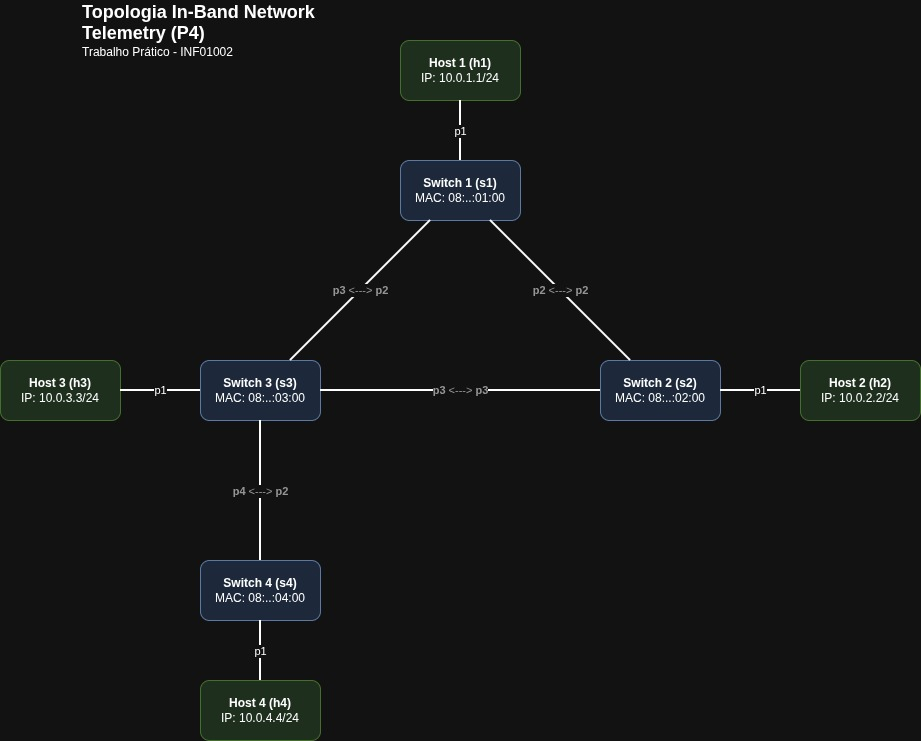
\includegraphics[width=0.8\textwidth]{figures/topologia_draw_io.jpg}
    \caption{Topologia da rede.}
\end{figure}

\begin{figure}[H]
    \centering
    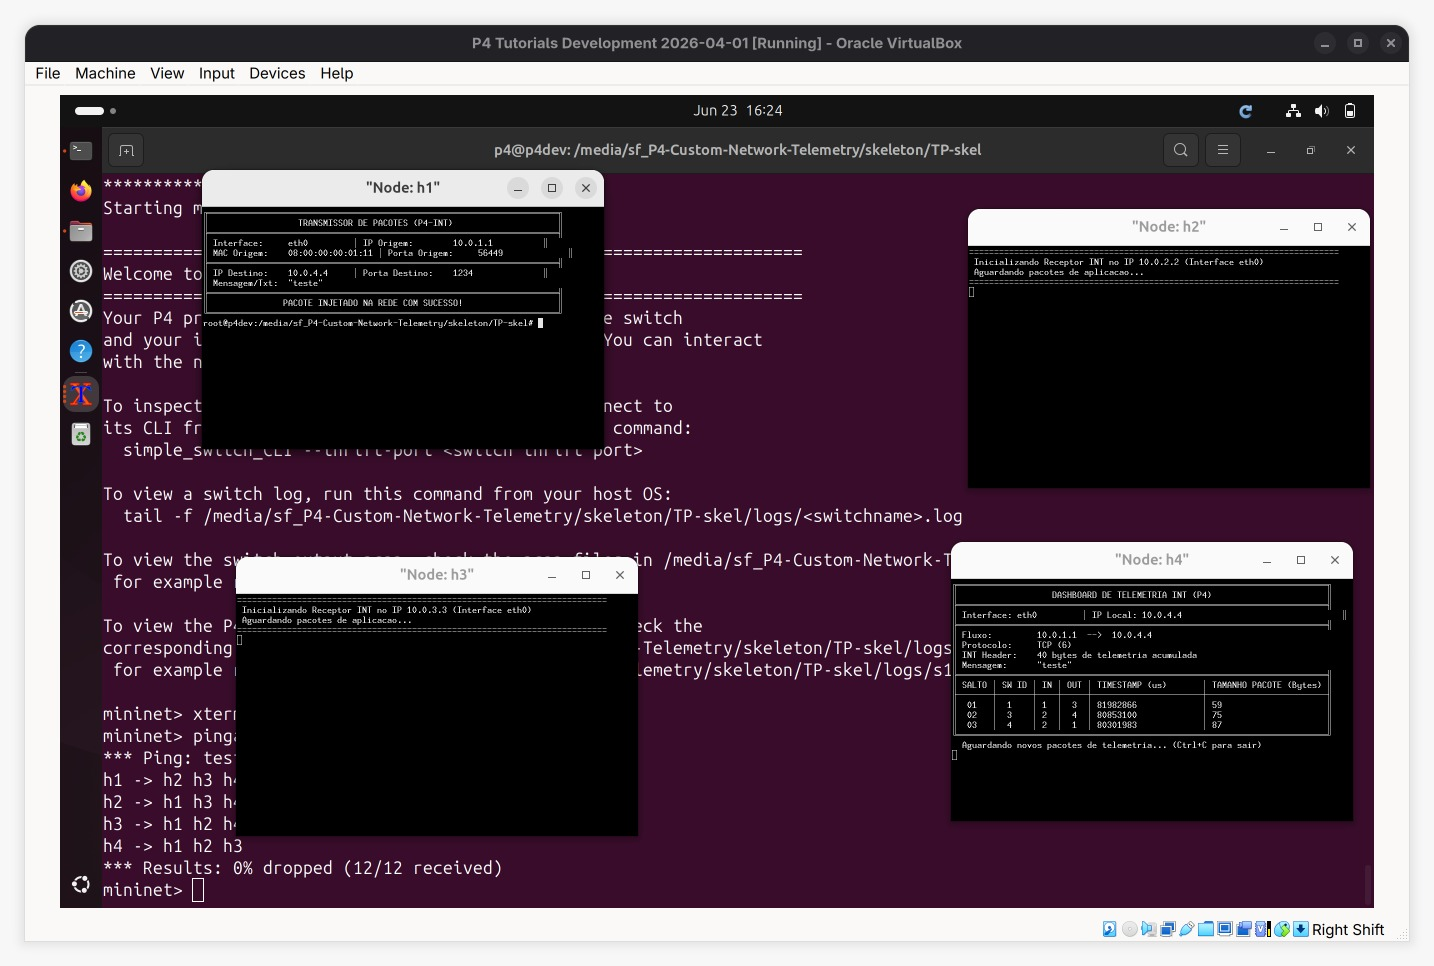
\includegraphics[width=0.8\textwidth]{figures/print.jpeg}
    \caption{Teste com 3 saltos.}
\end{figure}

Durante a extração dos dados na tabela TUI, observou-se que o \textit{timestamp} de um switch final no caminho pode apresentar valor inferior ao de um switch anterior. Esse comportamento comprova a natureza da simulação do BMv2 no Mininet, onde os processos não possuem sincronismo via \textit{Precision Time Protocol} (PTP), tornando os relógios independentes. Contudo, o acúmulo de saltos opera de forma contínua e robusta.


\section{Conclusão}
A implementação da \textit{In-Band Network Telemetry} (INT) em P4 provou ser um desafio técnico altamente enriquecedor, revelando as minúcias e complexidades operacionais inerentes ao plano de dados de redes programáveis.

Durante o desenvolvimento, diversas dificuldades técnicas foram encontradas, sendo a principal delas a interferência inicial da telemetria no tráfego de controle da rede (como os pacotes ICMP utilizados pelo comando \texttt{ping}).

Outro desafio significativo foi a atribuição de identificadores aos switches sem violar a regra de manter a topologia genérica e não adulterar o plano de controle (\textit{Control Plane}). 

Como ganho educacional, o trabalho consolidou de forma prática os conceitos de \textit{Software-Defined Networking} (SDN) e a separação dos planos de rede. Os conhecimentos sobre o encapsulamento estrutural de protocolos, a manipulação de pacotes byte a byte via código e a interação entre a camada de enlace e de rede foram aprofundados.

Por fim, a integração do plano de dados em P4 com a criação de \textit{dashboards} interativos via \textit{scripts} Python conectou a lógica de baixo nível dos switches BMv2 com a visualização de telemetria em alto nível. Isso proporcionou uma visão moderna de como monitoramento em tempo real.

\end{document}